\documentclass[12pt]{beamer}
\usepackage[english]{babel}
\usepackage{datetime}
\usepackage{tikz}
\usepackage{animate}
\usepackage{color}
\usepackage{colortbl}
\usetheme{Berlin}

\title[Employer Search and Screening in an Online Labor Market]{Employer Search and\\Screening in an Online\\Labor Market}
\author{John J. Horton}
\institute{oDesk Research}

\setbeamertemplate{footline}{%
  \begin{beamercolorbox}[sep=1mm,wd=\paperwidth,leftskip=1mm,rightskip=1mm]{footlinecolor}
    \hspace{1mm}%
    \tiny{\insertdate}
    \hfill
  \end{beamercolorbox}%
}

%gets rid of navigation symbols
\setbeamertemplate{navigation symbols}{}

\tikzstyle{every picture}+=[remember picture]
\tikzstyle{na} = [baseline=-.5ex]

\definecolor{myred}{RGB}{166,0,0}
\definecolor{gray100}{RGB}{0,0,0}
\definecolor{gray75}{RGB}{64,64,64}
\definecolor{gray50}{RGB}{128,128,128}
\definecolor{gray25}{RGB}{192,192,192}
\definecolor{gray0}{RGB}{255,255,255}
\definecolor{red100}{RGB}{255,0,0}
\definecolor{red75}{RGB}{255,64,64}
\definecolor{red50}{RGB}{255,128,128}
\definecolor{red25}{RGB}{255,192,192}
\definecolor{red0}{RGB}{255,255,255}

%our imaginary items - that is, placeholders for items
\newcommand*\imgitem{%
\item[\color{white}\scalebox{0.9}{\textbullet}]}

\newcommand*\imgitemtf{%
\item[\color{gray25}\scalebox{0.9}{\textbullet}]}

\newcommand*\imgitemfo{%
\item[\color{gray50}\scalebox{0.9}{\textbullet}]}

\newcommand*\imgitemsf{%
\item[\color{gray75}\scalebox{0.9}{\textbullet}]}

%our items
\newcommand*\ouritem{%
\item[\color{black}\scalebox{0.9}{\textbullet}]}

%our items
\newcommand*\variitem[1]{%
\item[\color{#1}\scalebox{0.9}{\textbullet}]}

\newcounter{boxes}
\setcounter{boxes}{1}

\newcommand\redbox[3]{%
\stepcounter{boxes}%
\begin{tikzpicture}[remember picture,overlay]
  \node[rectangle,rounded corners,line width=1pt,
      draw=myred,fill=myred!30,text height=20pt,
      text depth=11pt,align=left,fill opacity=0.7,text opacity=1] 
    (box-\theboxes) at #3 {#2};
  \node[rectangle,rounded corners,fill=myred!90,
      font={\Large\color{white}},anchor=west] 
    at ([xshift=10pt,]box-\theboxes.north west) {#1};
\end{tikzpicture}%
}

\newcommand\invbox[2]{%
\stepcounter{boxes}%
\begin{tikzpicture}[remember picture,overlay]
  \node 
    (box-\theboxes) at #2 {#1};
\end{tikzpicture}%
}

\begin{document}

\setlength{\baselineskip}{12mm}
\fontsize{10mm}{12mm}\selectfont

\begin{frame}
\begin{center}
Employer Search and\\
Screening in an Online\\
Labor Market

\vspace{3mm}

\large
John J. Horton\\
oDesk Research
\end{center}
\end{frame}

\begin{frame}{}
\begin{animateinline}[autoplay]{10}
\multiframe{5}{i=0+25}{
\begin{minipage}{\textwidth}
\begin{center}
\textcolor{gray\i}{Matching markets have}

\textcolor{gray\i}{search screening costs}
\end{center}
\end{minipage}
}
\end{animateinline}
\end{frame}

\begin{frame}{}
\begin{animateinline}[autoplay]{10}
\multiframe{5}{i=0+25}{
\begin{minipage}{\textwidth}
\Large
\begin{itemize}
\variitem{gray\i} \textcolor{gray\i}{What \emph{are} my options?}

\imgitem \textcolor{white}{\emph{How good} is each option for me?}
\end{itemize}
\end{minipage}
}
\newframe
\multiframe{5}{i=0+25}{
\begin{minipage}{\textwidth}
\Large
\begin{itemize}
\ouritem What \emph{are} my options?

\variitem{gray\i} \textcolor{gray\i}{\emph{How good} is each option for me?}
\end{itemize}
\end{minipage}
}
\end{animateinline}
\end{frame}

\begin{frame}{}
\begin{animateinline}[autoplay]{10}
\multiframe{5}{i=0+25}{
\begin{minipage}[c]{1\textwidth}
\begin{center}
\Large

\begin{figure}[H] \centering 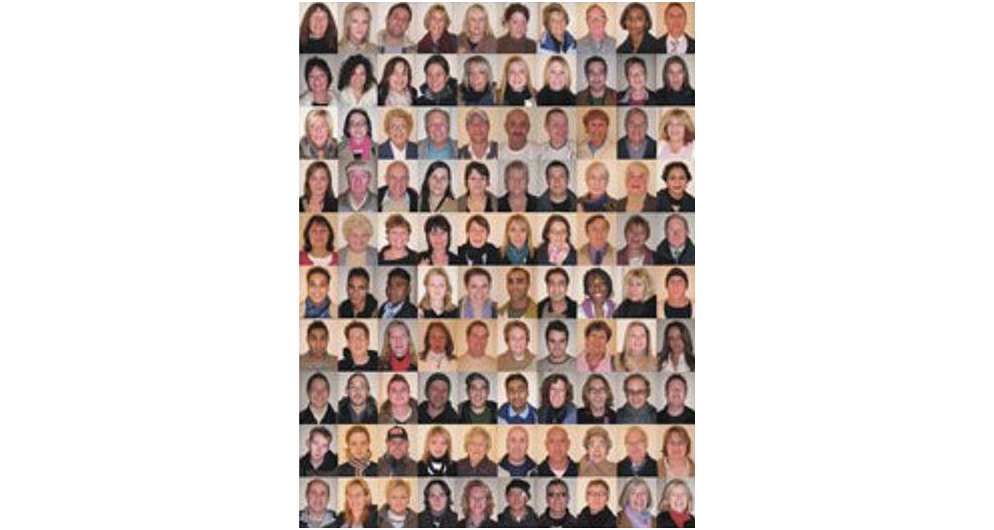
\includegraphics[width=100mm]{people_animation_1.png} \end{figure}

\textcolor{gray\i}{100 people}
\end{center}
\end{minipage}
}
\end{animateinline}
\end{frame}

\begin{frame}{}
\begin{animateinline}[autoplay]{10}
\multiframe{11}{i=1+1}{
\begin{minipage}[c]{1\textwidth}
\begin{center}
\Large

\begin{figure}[H] \centering \includegraphics[width=100mm]{people_animation_\i.png} \end{figure}

100 people
\end{center}
\end{minipage}
}
\newframe
\multiframe{9}{i=11+1}{
\begin{minipage}[c]{1\textwidth}
\begin{center}
\Large

\begin{figure}[H] \centering \includegraphics[width=100mm]{people_animation_\i.png} \end{figure}

1,000 people
\end{center}
\end{minipage}
}
\end{animateinline}
\end{frame}

\begin{frame}{}
\begin{animateinline}[autoplay]{10}
\multiframe{5}{i=1+1}{
\begin{minipage}[c]{1\textwidth}
\begin{center}
\Large

\begin{figure}[H] \centering \includegraphics[width=100mm]{people_animation_2_\i.png} \end{figure}

1,000 people
\end{center}
\end{minipage}
}
\newframe
\multiframe{6}{i=6+1}{
\begin{minipage}[c]{1\textwidth}
\begin{center}
\Large

\begin{figure}[H] \centering \includegraphics[width=100mm]{people_animation_2_\i.png} \end{figure}

100,000 people
\end{center}
\end{minipage}
}
\end{animateinline}
\end{frame}

\begin{frame}{}
\begin{animateinline}[autoplay]{10}
\multiframe{10}{i=1+1}{
\begin{minipage}[c]{1\textwidth}
\begin{center}
\Large

\begin{figure}[H] \centering \includegraphics[width=100mm]{people_animation_3_\i.png} \end{figure}

100,000 people
\end{center}
\end{minipage}
}
\newframe
\multiframe{8}{i=11+1}{
\begin{minipage}[c]{1\textwidth}
\begin{center}
\Large

\begin{figure}[H] \centering \includegraphics[width=100mm]{people_animation_3_\i.png} \end{figure}

1,000,000 people
\end{center}
\end{minipage}
}
\end{animateinline}
\end{frame}

\begin{frame}{}
\begin{animateinline}[autoplay]{10}
\multiframe{5}{i=0+25}{
\begin{minipage}{\textwidth}
\vspace{1 mm}
\begin{center}
\textcolor{gray\i}{Algorithmic approach}
\end{center}

\Large
\begin{itemize}
\imgitem \textcolor{white}{Infer nature of the work}

\imgitem \textcolor{white}{Find candidates with matching skills}

\imgitem \textcolor{white}{Sort matching candidates by some weighted combination of ability \& availability}
\end{itemize}
\end{minipage}
}
\newframe
\multiframe{5}{i=0+25}{
\begin{minipage}{\textwidth}
\vspace{1 mm}
\begin{center}
Algorithmic approach
\end{center}

\Large
\begin{itemize}
\variitem{gray\i} \textcolor{gray\i}{Infer nature of the work}

\imgitem \textcolor{white}{Find candidates with matching skills}

\imgitem \textcolor{white}{Sort matching candidates by some weighted combination of ability \& availability}
\end{itemize}
\end{minipage}
}
\newframe
\multiframe{5}{i=0+25}{
\begin{minipage}{\textwidth}
\vspace{1 mm}
\begin{center}
Algorithmic approach
\end{center}

\Large
\begin{itemize}
\ouritem Infer nature of the work

\variitem{gray\i} \textcolor{gray\i}{Find candidates with matching skills}

\imgitem \textcolor{white}{Sort matching candidates by some weighted combination of ability \& availability}
\end{itemize}
\end{minipage}
}
\newframe
\multiframe{5}{i=0+25}{
\begin{minipage}{\textwidth}
\vspace{1 mm}
\begin{center}
Algorithmic approach
\end{center}

\Large
\begin{itemize}
\ouritem Infer nature of the work

\ouritem Find candidates with matching skills

\variitem{gray\i} \textcolor{gray\i}{Sort matching candidates by some weighted combination of ability \& availability}
\end{itemize}
\end{minipage}
}
\end{animateinline}
\end{frame}

\begin{frame}{}
\begin{animateinline}[autoplay]{10}
\multiframe{5}{i=0+25}{
\begin{minipage}{\textwidth}
\vspace{1 mm}
\begin{center}
\textcolor{gray\i}{What segments matching}

\textcolor{gray\i}{markets traditionally?}
\end{center}

\Large
\begin{itemize}
\imgitem \textcolor{white}{Geography}

\imgitem \textcolor{white}{Time}

\imgitem \textcolor{white}{Costs of application}
\end{itemize}

\nointerlineskip
\begin{tikzpicture}[overlay]
\end{tikzpicture}
\end{minipage}
}
\newframe
\multiframe{5}{i=0+25}{
\begin{minipage}{\textwidth}
\vspace{1 mm}
\begin{center}
What segments matching

markets traditionally?
\end{center}

\Large
\begin{itemize}
\variitem{gray\i} \textcolor{gray\i}{Geography}

\imgitem \textcolor{white}{Time}

\imgitem \textcolor{white}{Costs of application}
\end{itemize}

\nointerlineskip
\begin{tikzpicture}[overlay]
\end{tikzpicture}
\end{minipage}
}
\newframe
\multiframe{5}{i=0+25}{
\begin{minipage}{\textwidth}
\vspace{1 mm}
\begin{center}
What segments matching

markets traditionally?
\end{center}

\Large
\begin{itemize}
\ouritem Geography

\variitem{gray\i} \textcolor{gray\i}{Time}

\imgitem \textcolor{white}{Costs of application}
\end{itemize}

\nointerlineskip
\begin{tikzpicture}[overlay]
\end{tikzpicture}
\end{minipage}
}
\newframe
\multiframe{5}{i=0+25}{
\begin{minipage}{\textwidth}
\vspace{1 mm}
\begin{center}
What segments matching

markets traditionally?
\end{center}

\Large
\begin{itemize}
\ouritem Geography

\ouritem Time

\variitem{gray\i} \textcolor{gray\i}{Costs of application}
\end{itemize}

\nointerlineskip
\begin{tikzpicture}[overlay]
\end{tikzpicture}
\end{minipage}
}
\newframe[20]
\begin{minipage}{\textwidth}
\vspace{1 mm}
\begin{center}
What segments matching

markets traditionally?
\end{center}

\Large
\begin{itemize}
\ouritem \tikz[na] \node[coordinate] (geo1) {};G\tikz[na] \node[coordinate] (geo2) {};eography

\ouritem Time

\ouritem Costs of application
\end{itemize}

\nointerlineskip
\begin{tikzpicture}[overlay]
\draw[line width=2pt,red] (geo1) edge [out=0, in=180] (geo2);
\end{tikzpicture}
\end{minipage}
\newframe
\begin{minipage}{\textwidth}
\vspace{1 mm}
\begin{center}
What segments matching

markets traditionally?
\end{center}

\Large
\begin{itemize}
\ouritem \tikz[na] \node[coordinate] (geo1) {};Ge\tikz[na] \node[coordinate] (geo2) {};ography

\ouritem Time

\ouritem Costs of application
\end{itemize}

\nointerlineskip
\begin{tikzpicture}[overlay]
\draw[line width=2pt,red] (geo1) edge [out=0, in=180] (geo2);
\end{tikzpicture}
\end{minipage}
\newframe
\begin{minipage}{\textwidth}
\vspace{1 mm}
\begin{center}
What segments matching

markets traditionally?
\end{center}

\Large
\begin{itemize}
\ouritem \tikz[na] \node[coordinate] (geo1) {};Geo\tikz[na] \node[coordinate] (geo2) {};graphy

\ouritem Time

\ouritem Costs of application
\end{itemize}

\nointerlineskip
\begin{tikzpicture}[overlay]
\draw[line width=2pt,red] (geo1) edge [out=0, in=180] (geo2);
\end{tikzpicture}
\end{minipage}
\newframe
\begin{minipage}{\textwidth}
\vspace{1 mm}
\begin{center}
What segments matching

markets traditionally?
\end{center}

\Large
\begin{itemize}
\ouritem \tikz[na] \node[coordinate] (geo1) {};Geog\tikz[na] \node[coordinate] (geo2) {};raphy

\ouritem Time

\ouritem Costs of application
\end{itemize}

\nointerlineskip
\begin{tikzpicture}[overlay]
\draw[line width=2pt,red] (geo1) edge [out=0, in=180] (geo2);
\end{tikzpicture}
\end{minipage}
\newframe
\begin{minipage}{\textwidth}
\vspace{1 mm}
\begin{center}
What segments matching

markets traditionally?
\end{center}

\Large
\begin{itemize}
\ouritem \tikz[na] \node[coordinate] (geo1) {};Geogr\tikz[na] \node[coordinate] (geo2) {};aphy

\ouritem Time

\ouritem Costs of application
\end{itemize}

\nointerlineskip
\begin{tikzpicture}[overlay]
\draw[line width=2pt,red] (geo1) edge [out=0, in=180] (geo2);
\end{tikzpicture}
\end{minipage}
\newframe
\begin{minipage}{\textwidth}
\vspace{1 mm}
\begin{center}
What segments matching

markets traditionally?
\end{center}

\Large
\begin{itemize}
\ouritem \tikz[na] \node[coordinate] (geo1) {};Geogra\tikz[na] \node[coordinate] (geo2) {};phy

\ouritem Time

\ouritem Costs of application
\end{itemize}

\nointerlineskip
\begin{tikzpicture}[overlay]
\draw[line width=2pt,red] (geo1) edge [out=0, in=180] (geo2);
\end{tikzpicture}
\end{minipage}
\newframe
\begin{minipage}{\textwidth}
\vspace{1 mm}
\begin{center}
What segments matching

markets traditionally?
\end{center}

\Large
\begin{itemize}
\ouritem \tikz[na] \node[coordinate] (geo1) {};Geograp\tikz[na] \node[coordinate] (geo2) {};hy

\ouritem Time

\ouritem Costs of application
\end{itemize}

\nointerlineskip
\begin{tikzpicture}[overlay]
\draw[line width=2pt,red] (geo1) edge [out=0, in=180] (geo2);
\end{tikzpicture}
\end{minipage}
\newframe
\begin{minipage}{\textwidth}
\vspace{1 mm}
\begin{center}
What segments matching

markets traditionally?
\end{center}

\Large
\begin{itemize}
\ouritem \tikz[na] \node[coordinate] (geo1) {};Geograph\tikz[na] \node[coordinate] (geo2) {};y

\ouritem Time

\ouritem Costs of application
\end{itemize}

\nointerlineskip
\begin{tikzpicture}[overlay]
\draw[line width=2pt,red] (geo1) edge [out=0, in=180] (geo2);
\end{tikzpicture}
\end{minipage}
\newframe
\begin{minipage}{\textwidth}
\vspace{1 mm}
\begin{center}
What segments matching

markets traditionally?
\end{center}

\Large
\begin{itemize}
\ouritem \tikz[na] \node[coordinate] (geo1) {};Geography\tikz[na] \node[coordinate] (geo2) {};

\ouritem Time

\ouritem Costs of application
\end{itemize}

\nointerlineskip
\begin{tikzpicture}[overlay]
\draw[line width=2pt,red] (geo1) edge [out=0, in=180] (geo2);
\end{tikzpicture}
\end{minipage}
\newframe[10]
\multiframe{5}{i=0+25}{
\begin{minipage}{\textwidth}
\vspace{1 mm}
\begin{center}
What segments matching

markets traditionally?
\end{center}

\Large
\begin{itemize}
\ouritem \tikz[na] \node[coordinate] (geo1) {};Geography\tikz[na] \node[coordinate] (geo2) {}; 
\invbox{
\small
\textcolor{red\i}{No inherent geographic constraints}}{(0.3\textwidth,0.025\textheight)}
\invbox{
\small
\textcolor{red\i}{in online labor markets}}{(0.3\textwidth,-0.025\textheight)}

\ouritem Time

\ouritem Costs of application
\end{itemize}

\nointerlineskip
\begin{tikzpicture}[overlay]
\draw[line width=2pt,red] (geo1) edge [out=0, in=180] (geo2);
\end{tikzpicture}
\end{minipage}
}
\end{animateinline}
\end{frame}

\begin{frame}{}
\begin{animateinline}[autoplay]{10}
\multiframe{5}{i=0+25}{
\begin{minipage}{\textwidth}
\vspace{1 mm}
\begin{center}
\textcolor{gray\i}{Search and scale}
\end{center}

\Large
\begin{itemize}
\imgitem \textcolor{white}{Effects of scale}

\begin{itemize}
\Large
\imgitem \textcolor{white}{Plus: More space for higher-quality matches}

\imgitem \textcolor{white}{Negative: The {\grqq}what are'' and {\grqq}how good are'' questions about options get harder with scale}
\end{itemize}
\end{itemize}
\end{minipage}
}
\newframe
\multiframe{5}{i=0+25}{
\begin{minipage}{\textwidth}
\vspace{1 mm}
\begin{center}
Search and scale
\end{center}

\Large
\begin{itemize}
\variitem{gray\i} \textcolor{gray\i}{Effects of scale}

\begin{itemize}
\Large
\imgitem \textcolor{white}{Plus: More space for higher-quality matches}

\imgitem \textcolor{white}{Negative: The {\grqq}what are'' and {\grqq}how good are'' questions about options get harder with scale}
\end{itemize}
\end{itemize}
\end{minipage}
}
\newframe
\multiframe{5}{i=0+25}{
\begin{minipage}{\textwidth}
\vspace{1 mm}
\begin{center}
Search and scale
\end{center}

\Large
\begin{itemize}
\ouritem Effects of scale

\begin{itemize}
\Large
\variitem{gray\i} \textcolor{gray\i}{Plus: More space for higher-quality matches}

\imgitem \textcolor{white}{Negative: The {\grqq}what are'' and {\grqq}how good are'' questions about options get harder with scale}
\end{itemize}
\end{itemize}
\end{minipage}
}
\newframe
\multiframe{5}{i=0+25}{
\begin{minipage}{\textwidth}
\vspace{1 mm}
\begin{center}
Search and scale
\end{center}

\Large
\begin{itemize}
\ouritem Effects of scale

\begin{itemize}
\Large
\ouritem Plus: More space for higher-quality matches

\variitem{gray\i} \textcolor{gray\i}{Negative: The {\grqq}what are'' and {\grqq}how good are'' questions about options get harder with scale}
\end{itemize}
\end{itemize}
\end{minipage}
}
\end{animateinline}
\end{frame}

\begin{frame}{}
\begin{animateinline}[autoplay]{10}
\multiframe{5}{i=0+25}{
\begin{minipage}{\textwidth}
\Large
\vspace{1 mm}
\begin{itemize}
\variitem{gray\i} \textcolor{gray\i}{To what extent can we subsidize search and screening algorithmically, and is this subsidization effective?}
\end{itemize}
\end{minipage}
}
\end{animateinline}
\end{frame}

\begin{frame}{}
\begin{animateinline}[autoplay]{10}
\multiframe{5}{i=0+25}{
\begin{minipage}{\textwidth}
\begin{center}
\vspace{1 mm}
\textcolor{gray\i}{Can these costs be reduced by third-parties?}
\end{center}
\end{minipage}
}
\end{animateinline}
\end{frame}

\begin{frame}{}
\begin{animateinline}[autoplay]{10}
\multiframe{5}{i=0+25}{
\begin{minipage}{\textwidth}
\begin{center}
\textcolor{gray\i}{Labor market examples}
\end{center}

\Large
\vspace{1 mm}
\begin{itemize}
\imgitem \textcolor{white}{Credentialing services}

\imgitem \textcolor{white}{Unions}

\imgitem \textcolor{white}{Information clearing-houses}

\imgitem \textcolor{white}{Job-listing sites}

\imgitem \textcolor{white}{Placement services}

\begin{itemize}
\Large
\imgitem \textcolor{white}{E.g., counseling, recommendations}
\end{itemize}
\end{itemize}
\end{minipage}
}
\newframe
\multiframe{5}{i=0+25}{
\begin{minipage}{\textwidth}
\begin{center}
Labor market examples
\end{center}

\Large
\vspace{1 mm}
\begin{itemize}
\variitem{gray\i} \textcolor{gray\i}{Credentialing services}

\imgitem \textcolor{white}{Unions}

\imgitem \textcolor{white}{Information clearing-houses}

\imgitem \textcolor{white}{Job-listing sites}

\imgitem \textcolor{white}{Placement services}

\begin{itemize}
\Large
\imgitem \textcolor{white}{E.g., counseling, recommendations}
\end{itemize}
\end{itemize}
\end{minipage}
}
\newframe
\multiframe{5}{i=0+25}{
\begin{minipage}{\textwidth}
\begin{center}
Labor market examples
\end{center}

\Large
\vspace{1 mm}
\begin{itemize}
\variitem{gray100} \textcolor{gray100}{Credentialing services}

\variitem{gray\i} \textcolor{gray\i}{Unions}

\imgitem \textcolor{white}{Information clearing-houses}

\imgitem \textcolor{white}{Job-listing sites}

\imgitem \textcolor{white}{Placement services}

\begin{itemize}
\Large
\imgitem \textcolor{white}{E.g., counseling, recommendations}
\end{itemize}
\end{itemize}
\end{minipage}
}
\newframe
\multiframe{5}{i=0+25}{
\begin{minipage}{\textwidth}
\begin{center}
Labor market examples
\end{center}

\Large
\vspace{1 mm}
\begin{itemize}
\variitem{gray100} \textcolor{gray100}{Credentialing services}

\variitem{gray100} \textcolor{gray100}{Unions}

\variitem{gray\i} \textcolor{gray\i}{Information clearing-houses}

\imgitem \textcolor{white}{Job-listing sites}

\imgitem \textcolor{white}{Placement services}

\begin{itemize}
\Large
\imgitem \textcolor{white}{E.g., counseling, recommendations}
\end{itemize}
\end{itemize}
\end{minipage}
}
\newframe
\multiframe{5}{i=0+25}{
\begin{minipage}{\textwidth}
\begin{center}
Labor market examples
\end{center}

\Large
\vspace{1 mm}
\begin{itemize}
\variitem{gray100} \textcolor{gray100}{Credentialing services}

\variitem{gray100} \textcolor{gray100}{Unions}

\variitem{gray100} \textcolor{gray100}{Information clearing-houses}

\variitem{gray\i} \textcolor{gray\i}{Job-listing sites}

\imgitem \textcolor{white}{Placement services}

\begin{itemize}
\Large
\imgitem \textcolor{white}{E.g., counseling, recommendations}
\end{itemize}
\end{itemize}
\end{minipage}
}
\newframe
\multiframe{5}{i=0+25}{
\begin{minipage}{\textwidth}
\begin{center}
Labor market examples
\end{center}

\Large
\vspace{1 mm}
\begin{itemize}
\variitem{gray100} \textcolor{gray100}{Credentialing services}

\variitem{gray100} \textcolor{gray100}{Unions}

\variitem{gray100} \textcolor{gray100}{Information clearing-houses}

\variitem{gray100} \textcolor{gray100}{Job-listing sites}

\variitem{gray\i} \textcolor{gray\i}{Placement services}

\begin{itemize}
\Large
\imgitem \textcolor{white}{E.g., counseling, recommendations}
\end{itemize}
\end{itemize}
\end{minipage}
}
\newframe
\multiframe{5}{i=0+25}{
\begin{minipage}{\textwidth}
\begin{center}
Labor market examples
\end{center}

\Large
\vspace{1 mm}
\begin{itemize}
\variitem{gray100} \textcolor{gray100}{Credentialing services}

\variitem{gray100} \textcolor{gray100}{Unions}

\variitem{gray100} \textcolor{gray100}{Information clearing-houses}

\variitem{gray100} \textcolor{gray100}{Job-listing sites}

\variitem{gray100} \textcolor{gray100}{Placement services}

\begin{itemize}
\Large
\variitem{gray\i} \textcolor{gray\i}{E.g., counseling, recommendations}
\end{itemize}
\end{itemize}
\end{minipage}
}
\end{animateinline}
\end{frame}

\begin{frame}{}
\begin{animateinline}[autoplay]{10}
\multiframe{5}{i=0+25}{
\begin{minipage}{\textwidth}
\begin{center}
\vspace{1 mm}
\textcolor{gray\i}{Main concern with any targeted assistance?}

\textcolor{white}{\emph{Crowd-out}}
\vspace{1 mm}
\end{center}
\end{minipage}
}
\newframe
\multiframe{5}{i=0+25}{
\begin{minipage}{\textwidth}
\begin{center}
\vspace{1 mm}
Main concern with any targeted assistance?

\textcolor{gray\i}{\emph{Crowd-out}}
\vspace{1 mm}
\end{center}
\end{minipage}
}
\end{animateinline}
\end{frame}

\begin{frame}{}
\begin{animateinline}[autoplay]{10}
\multiframe{5}{i=0+25}{
\begin{minipage}{\textwidth}
\begin{center}
\Large
\textcolor{gray\i}{Two engineers, Alice \& Bob}

\textcolor{gray0}{Two vacancies at Facebook \& Twitter}

\textcolor{gray0}{Each has match-specific productivities}

\textcolor{gray0}{Only one worker per vacancy}

\textcolor{gray0}{We ignore bargaining}

\vspace{10 mm}

\begin{tabular}{!{\color{gray0}\vrule} c !{\color{gray0}\vrule} c !{\color{gray0}\vrule} c !{\color{gray0}\vrule}}
\arrayrulecolor{gray0}\hline
 & \textcolor{gray0}{Alice} & \textcolor{gray0}{Bob} \\
\arrayrulecolor{gray0}\hline
 \textcolor{gray0}{Twitter} & \textcolor{gray0}{8} & \textcolor{gray0}{12} \\
\arrayrulecolor{gray0}\hline
 \textcolor{gray0}{Facebook} & \textcolor{gray0}{10} & \textcolor{gray0}{20} \\
\arrayrulecolor{gray0}\hline
\end{tabular}
\end{center}
\end{minipage}
}
\newframe
\multiframe{5}{i=0+25}{
\begin{minipage}{\textwidth}
\begin{center}
\Large
\textcolor{gray100}{Two engineers, Alice \& Bob}

\textcolor{gray\i}{Two vacancies at Facebook \& Twitter}

\textcolor{gray0}{Each has match-specific productivities}

\textcolor{gray0}{Only one worker per vacancy}

\textcolor{gray0}{We ignore bargaining}

\vspace{10 mm}

\begin{tabular}{!{\color{gray0}\vrule} c !{\color{gray0}\vrule} c !{\color{gray0}\vrule} c !{\color{gray0}\vrule}}
\arrayrulecolor{gray0}\hline
 & \textcolor{gray0}{Alice} & \textcolor{gray0}{Bob} \\
\arrayrulecolor{gray0}\hline
 \textcolor{gray0}{Twitter} & \textcolor{gray0}{8} & \textcolor{gray0}{12} \\
\arrayrulecolor{gray0}\hline
 \textcolor{gray0}{Facebook} & \textcolor{gray0}{10} & \textcolor{gray0}{20} \\
\arrayrulecolor{gray0}\hline
\end{tabular}
\end{center}
\end{minipage}
}
\newframe
\multiframe{5}{i=0+25}{
\begin{minipage}{\textwidth}
\begin{center}
\Large
\textcolor{gray100}{Two engineers, Alice \& Bob}

\textcolor{gray100}{Two vacancies at Facebook \& Twitter}

\textcolor{gray\i}{Each has match-specific productivities}

\textcolor{gray0}{Only one worker per vacancy}

\textcolor{gray0}{We ignore bargaining}

\vspace{10 mm}

\begin{tabular}{!{\color{gray0}\vrule} c !{\color{gray0}\vrule} c !{\color{gray0}\vrule} c !{\color{gray0}\vrule}}
\arrayrulecolor{gray0}\hline
 & \textcolor{gray0}{Alice} & \textcolor{gray0}{Bob} \\
\arrayrulecolor{gray0}\hline
 \textcolor{gray0}{Twitter} & \textcolor{gray0}{8} & \textcolor{gray0}{12} \\
\arrayrulecolor{gray0}\hline
 \textcolor{gray0}{Facebook} & \textcolor{gray0}{10} & \textcolor{gray0}{20} \\
\arrayrulecolor{gray0}\hline
\end{tabular}
\end{center}
\end{minipage}
}
\newframe
\multiframe{5}{i=0+25}{
\begin{minipage}{\textwidth}
\begin{center}
\Large
\textcolor{gray100}{Two engineers, Alice \& Bob}

\textcolor{gray100}{Two vacancies at Facebook \& Twitter}

\textcolor{gray100}{Each has match-specific productivities}

\textcolor{gray\i}{Only one worker per vacancy}

\textcolor{gray0}{We ignore bargaining}

\vspace{10 mm}

\begin{tabular}{!{\color{gray0}\vrule} c !{\color{gray0}\vrule} c !{\color{gray0}\vrule} c !{\color{gray0}\vrule}}
\arrayrulecolor{gray0}\hline
 & \textcolor{gray0}{Alice} & \textcolor{gray0}{Bob} \\
\arrayrulecolor{gray0}\hline
 \textcolor{gray0}{Twitter} & \textcolor{gray0}{8} & \textcolor{gray0}{12} \\
\arrayrulecolor{gray0}\hline
 \textcolor{gray0}{Facebook} & \textcolor{gray0}{10} & \textcolor{gray0}{20} \\
\arrayrulecolor{gray0}\hline
\end{tabular}
\end{center}
\end{minipage}
}
\newframe
\multiframe{5}{i=0+25}{
\begin{minipage}{\textwidth}
\begin{center}
\Large
\textcolor{gray100}{Two engineers, Alice \& Bob}

\textcolor{gray100}{Two vacancies at Facebook \& Twitter}

\textcolor{gray100}{Each has match-specific productivities}

\textcolor{gray100}{Only one worker per vacancy}

\textcolor{gray\i}{We ignore bargaining}

\vspace{10 mm}

\begin{tabular}{!{\color{gray0}\vrule} c !{\color{gray0}\vrule} c !{\color{gray0}\vrule} c !{\color{gray0}\vrule}}
\arrayrulecolor{gray0}\hline
 & \textcolor{gray0}{Alice} & \textcolor{gray0}{Bob} \\
\arrayrulecolor{gray0}\hline
 \textcolor{gray0}{Twitter} & \textcolor{gray0}{8} & \textcolor{gray0}{12} \\
\arrayrulecolor{gray0}\hline
 \textcolor{gray0}{Facebook} & \textcolor{gray0}{10} & \textcolor{gray0}{20} \\
\arrayrulecolor{gray0}\hline
\end{tabular}
\end{center}
\end{minipage}
}
\newframe
\multiframe{5}{i=0+25}{
\begin{minipage}{\textwidth}
\begin{center}
\Large
Two engineers, Alice \& Bob

Two vacancies at Facebook \& Twitter

Each has match-specific productivities

Only one worker per vacancy

We ignore bargaining

\vspace{10 mm}

\begin{tabular}{!{\color{gray\i}\vrule} c !{\color{gray\i}\vrule} c !{\color{gray\i}\vrule} c !{\color{gray\i}\vrule}}
\arrayrulecolor{gray\i}\hline
 & \textcolor{gray\i}{Alice} & \textcolor{gray\i}{Bob} \\
\arrayrulecolor{gray\i}\hline
 \textcolor{gray\i}{Twitter} & \textcolor{gray\i}{8} & \textcolor{gray\i}{12} \\
\arrayrulecolor{gray\i}\hline
 \textcolor{gray\i}{Facebook} & \textcolor{gray\i}{10} & \textcolor{gray\i}{20} \\
\arrayrulecolor{gray\i}\hline
\end{tabular}
\end{center}
\end{minipage}
}
\end{animateinline}
\end{frame}

\end{document}